\documentclass[11pt,twoside,a4paper]{article}
\usepackage[utf8]{inputenc}
\usepackage{titlesec}
\usepackage[hidelinks]{hyperref}
\usepackage{pdfpages}

\newcommand{\sectionbreak}{\clearpage}
\renewcommand\contentsname{Inhaltsverzeichnis}

\begin{document}
\pagenumbering{roman}
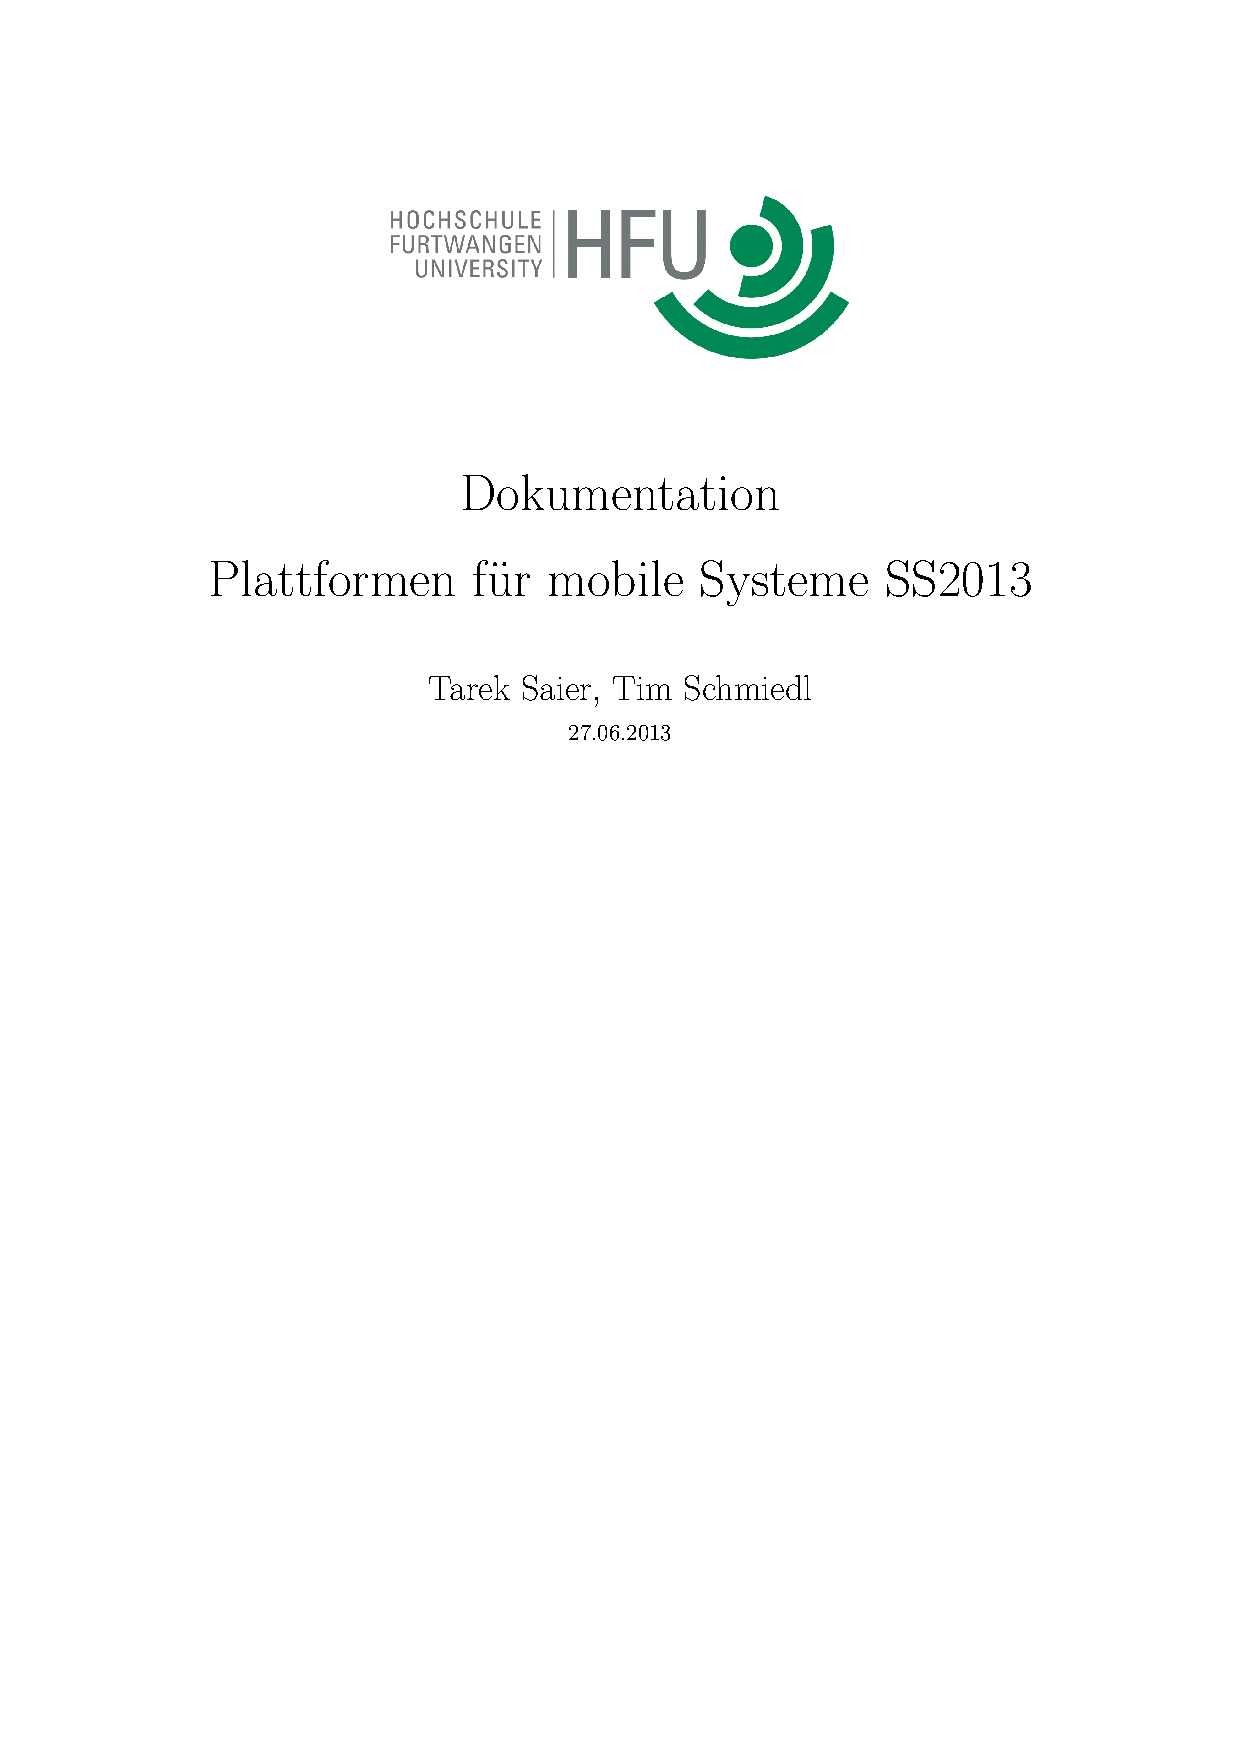
\includepdf{titlepage.pdf}

\clearpage
\setcounter{page}{1}
\tableofcontents

\section{Aufgabenstellung}
\pagenumbering{arabic}
\setcounter{page}{1}
Die Aufgabenstellung bestand darin, den Bootvorgang des Pandaboards so zu gestaltet, dass der Kernel im Kontext des U-Boot Bootloaders\footnote{\url{http://www.denx.de/wiki/U-Boot}} via TFTP geladen wird. Es soll sich also kein Kernel auf der SD-Karte des Boards befinden.

\section{Umsetzung}
\subsection{TFTP}
\begin{itemize}
	\item Nach Anleitung\footnote{\url{http://processors.wiki.ti.com/index.php/Booting\_Linux\_kernel\_using\_U-Boot}}
	\item atftpd = fail
	\item tftpd-hpa = get funktioneirt
\end{itemize}
\subsection{U-Boot}
\begin{itemize}
	\item \textbf{Kein Ethernet}\\
	\begin{verbatim}
	...

	Using default evnironment
	
	In: serial
	Out: serial
	Err: serial
	Net: No ethernet found.
	checking for preEnv.txt

	...
	\end{verbatim}
	\item \textbf{Ethernet aber keine Möglichkeit es zu verifizieren}\\ 
	wie oben nur \texttt{NET: KS8851SNL}
\end{itemize}
\end{document}
